\documentclass[12pt, a4paper]{report}
\usepackage[utf8]{inputenc} % Eingabekodierung
\usepackage[T1]{fontenc} % Fontkodierung
\usepackage[english]{babel} % Deutsche Sprache
\usepackage{graphicx} % Grafiken
\usepackage{hyperref} % Hyperlinks
\usepackage{geometry} % Seitenlayout
\usepackage{setspace} % Zeilenabstand
\usepackage{fancyhdr} % Kopf- und Fußzeile
\usepackage{titlesec} % Kapitelnummerierung
\usepackage{adjustbox} % Bildbearbeitung
\usepackage{subcaption}
\usepackage{titletoc}
\usepackage[backend=biber, style=authoryear, maxcitenames=1, mincitenames=1]{biblatex}
\addbibresource{2023_11_29_Seminararbeit.bib}

\geometry{a4paper, margin=2.5cm} % Seitenränder
\hypersetup{colorlinks=true, urlcolor=blue, linkcolor=black, citecolor=black} % Hyperlinks einrichten
\onehalfspacing % Zeilenabstand auf 1,5-fach setzen

\usepackage{enumitem} % Formatierung Aufzählungsverzeichnis enumerate

\makeatletter
\renewcommand{\@roman}[1]{\expandafter\@slowromancap\romannumeral #1@}
\makeatother

\usepackage[printonlyused]{acronym}

\usepackage{glossaries}
\newglossaryentry{symb:A}{
	name={\(A\)},
	description={Beschreibung des Symbols \(A\)}
}
\newglossaryentry{symb:B}{
	name={\(B\)},
	description={Beschreibung des Symbols \(B\)}
}
\makeglossaries

\pagestyle{fancy}
\fancyhf{} % Löscht alle voreingestellten Kopf- und Fußzeileneinstellungen

% Definiere die Kopfzeile
\lhead{\leftmark} % Aktuelles Kapitel auf der linken Seite
\chead{} % Kein Inhalt in der Mitte der Kopfzeile
\rhead{} % Kein Inhalt auf der rechten Seite der Kopfzeile

% Definiere die Fußzeile (optional)
\lfoot{} % Kein Inhalt auf der linken Seite der Fußzeile
\cfoot{\thepage} % Seitenzahl in der Mitte der Fußzeile
\rfoot{} % Kein Inhalt auf der rechten Seite der Fußzeile

\DeclareNameAlias{sortname}{last-first}
\renewcommand*{\nameyeardelim}{\addcomma\addspace}

%Formatierung für Online-Zitate
\DeclareCiteCommand{\citeonline}[\mkbibparens]
{\usebibmacro{prenote}}
{\usebibmacro{citeindex}%
	\printtext[bibhyperref]{%
		\printfield{title}%
		\setunit{\addcomma\space}%
		\printfield{year}}}
{\multicitedelim}
{\usebibmacro{postnote}}

\titleformat{\chapter}[hang]
{\normalfont\huge\bfseries}{\thechapter.}{0.5em}{\huge\bfseries}

\renewcommand{\figurename}{Figure}

\begin{document}

\begin{titlepage}
	\centering
	
\includegraphics[width=0.5\textwidth]{2023_11_29_Bilder_Dokumentation/hhn-logo.png}

	\vspace*{15mm}

	{\LARGE \textbf{Faculty of Engineering (TE)\\Automotive Systems Engineering}}

	\vspace*{15mm}

	{\Huge Project for Digital Signal Processing}

	\vspace*{15mm}

	{\Large Project Documentation}\\
	Master Automotive Systems Engineering\\

	by\\

	{\Large Jakob Kurz \& Mattis Tom Ritter}\\
	(Matriculation-Nr. 210262 \& 210265)\\

	\vspace{5mm}

	presented in Wintersemester 2024/25 at\\

	\vspace{5mm}

	{\Large Heilbronn University}

	\vspace*{10mm}

	\begin{tabbing}
		\hspace*{4cm}Reviewer: \hspace*{1cm}\=Prof. Dr. Volker Stahl\\
		\hspace*{4cm}Levy: \>31. December 2024
	\end{tabbing}
\end{titlepage}


\pagenumbering{gobble} % Ausschalten der Seitennummerierung

\renewcommand{\contentsname}{Table of Contents}
\tableofcontents % Inhaltsverzeichnis erstellen
\newpage

\pagenumbering{roman} % Verzeichnisse werden in römischen zahlen nummeriert´

\chapter*{List of Abbreviations}
\label{sec:abkuerzungsverzeichnis}
\begin{acronym}[OpenCV]
	\acro{DFT}{Discrete Fourier Transform}
	\acro{FFT}{Fast Fourier Transform}
\end{acronym}
\newpage

\renewcommand{\listfigurename}{List of Figures}
\listoffigures
\newpage

%\listoftables
%\newpage

%\subsection*{Symbolverzeichnis}
%\label{sec:symbolverzeichnis}
%\printglossary
%\newpage

\pagenumbering{arabic}
\setcounter{page}{1}	% Setze Seitenzähler auf 1

\chapter{Basic Implementations}

\section{\ac{DFT} vs. \ac{FFT}}

\subsection{Implementation Overview}
The implementations of the \ac{DFT} and \ac{FFT} are provided in the files \texttt{dft.py} and \texttt{fft.py}, respectively. The \ac{DFT} computes the Fourier Transform by performing a matrix-vector multiplication using the complex-valued matrix \( B \). This matrix represents the discrete Fourier kernel, with elements defined as \( B[k, l] = e^{-2\pi i k l / N} \). The \ac{DFT} directly calculates the transform by multiplying the input vector \( f \) with \( B \), resulting in a computational complexity of \(O(N^2)\).\\
In contrast, the FFT optimizes the Fourier Transform computation by reducing the complexity to \(O(N \log N)\). The recursive FFT employs a divide-and-conquer approach, splitting the input signal into smaller subproblems and recursively computing the transform. The iterative FFT further optimizes this process by eliminating recursion and using butterfly operations, which enable efficient in-place computations.

\subsection{Testing and Verification}
The correctness of the \ac{DFT} and \ac{FFT} implementations is validated through comprehensive testing, focusing on both individual and comparative evaluations of the methods.

\subsubsection{Tests for Individual Implementations}
The tests in \texttt{test\_dft.py} verify the correctness of the \ac{DFT} and its optimized variants. These include reconstructing random real and complex signals using the inverse \ac{DFT} (IDFT), ensuring that \( \text{IDFT}(\text{DFT}(f)) = f \) and \( \text{DFT}(\text{IDFT}(z)) = z \). Additional tests compare the outputs of the standard and optimized implementations, as well as against NumPy's FFT. A cosine wave test checks the magnitude of the transformed coefficients against expected values.\\
Similarly, \texttt{test\_fft.py} evaluates both the recursive and iterative FFT implementations. Tests confirm equivalence with NumPy's FFT results for real and complex signals, ensure that \( \text{IFFT}(\text{FFT}(f)) = f \), and verify that the recursive and iterative FFT produce identical outputs. These tests validate the accuracy and consistency of each implementation.

\subsubsection{Comparative Testing of \ac{DFT} and \ac{FFT}}
The script \texttt{test\_dft\_fft.py} compares the \ac{DFT} with the recursive and iterative FFT. A sinusoidal test signal is processed by all three methods, and their outputs are compared element-wise within a tolerance of \(10^{-9}\). This ensures numerical equivalence between the methods, confirming that the \ac{DFT} and FFT implementations produce consistent results.

\subsection{Verification of Similarities}
The script \texttt{vis\_dft\_fft\_simmiliar.py} visualizes the similarities between the methods. In the frequency domain, all methods accurately identify the signal's frequency components. However, only half of the spectrum is shown due to the symmetry inherent to real-valued signals (see Fig. \ref{fig:frequency_domain_comparison} left). In the time domain, all methods reconstruct the original signal with minimal deviations (see Fig. \ref{fig:frequency_domain_comparison} right).

\begin{figure}[h!]
	\centering
	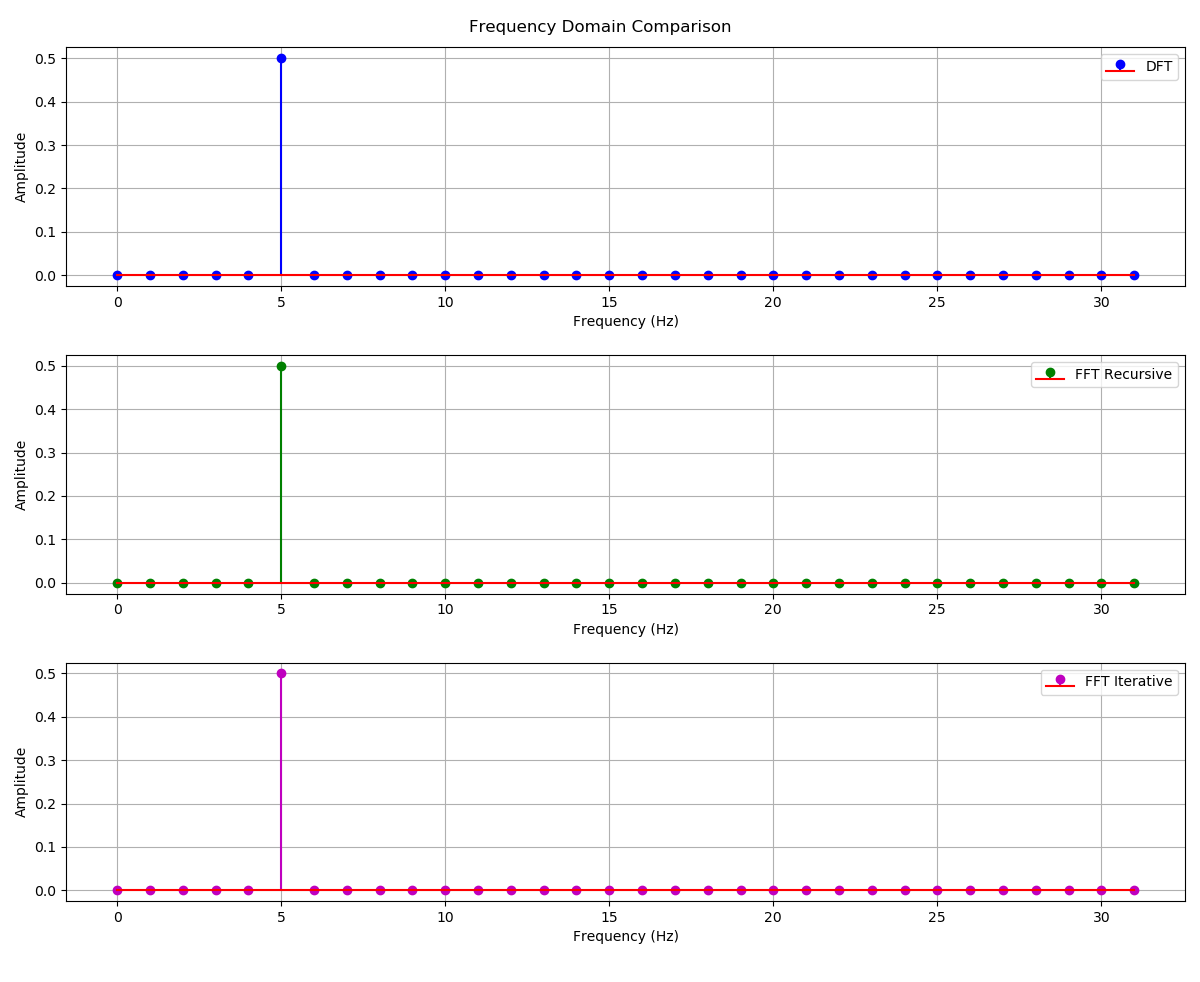
\includegraphics[width=0.45\textwidth]{2023_11_29_Bilder_Dokumentation/Frequency_Domain_Comparison.png}
	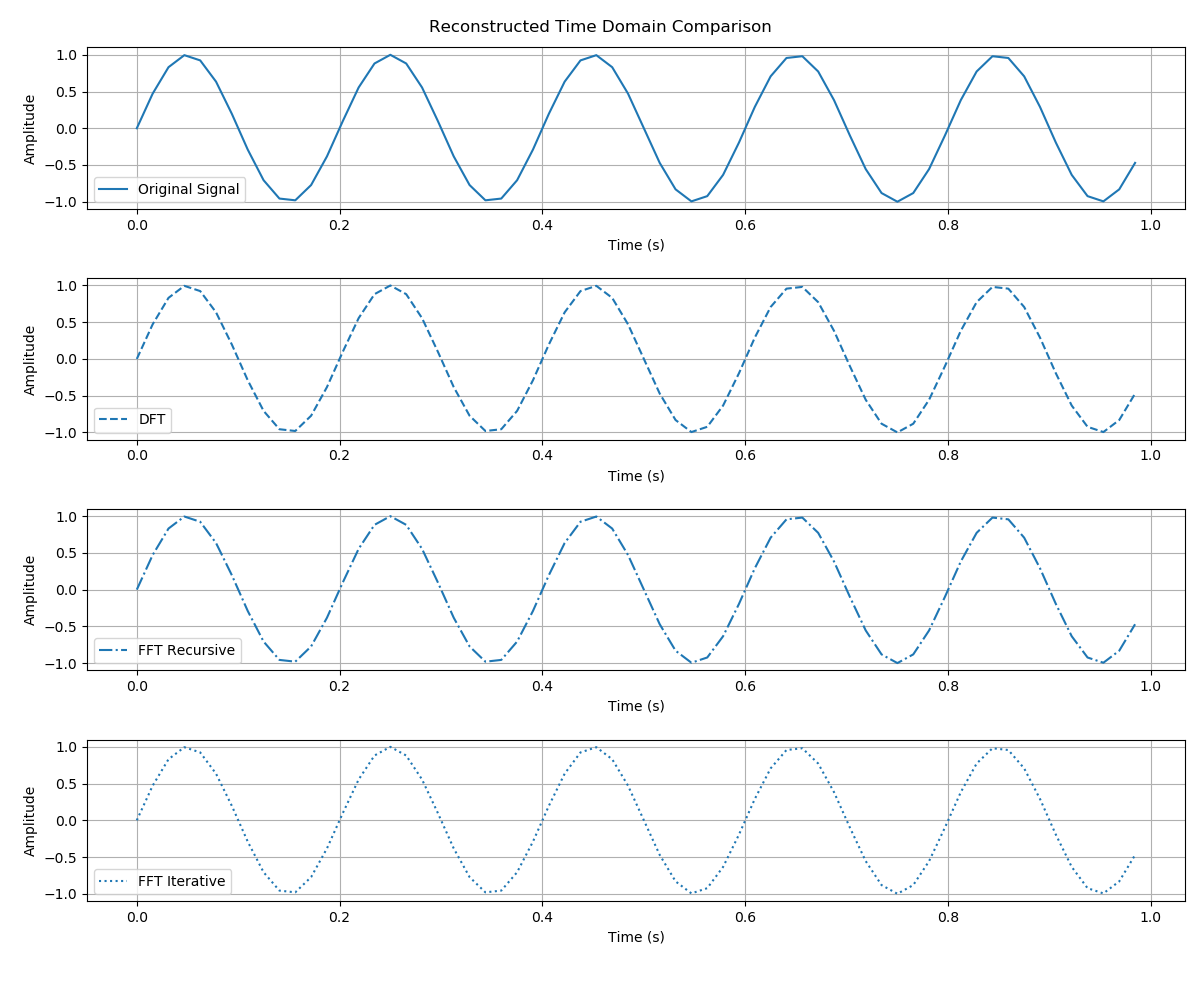
\includegraphics[width=0.45\textwidth]{2023_11_29_Bilder_Dokumentation/Time_Domain_Comparison.png}
	\caption{Frequency domain comparison (left) and Time-domain reconstruction validation (right)}
	\label{fig:frequency_domain_comparison}
\end{figure}

\subsection{Comparison of Differences}
To highlight differences, the script \texttt{vis\_dft\_fft\_different.py} visualizes the computational time and memory usage for the \ac{DFT} and \ac{FFT}.\\
Figure \ref{fig:time_memory_comparison} compares execution time and memory usage for a fixed signal length. The \ac{DFT} requires significantly more time due to its quadratic complexity of \(O(N^2)\), while both \ac{FFT} implementations achieve logarithmic complexity of \(O(N \log N)\). The recursive FFT is slightly faster than the iterative FFT in this case. Regarding memory usage, the iterative FFT is the most efficient, whereas the recursive FFT demands more due to its reliance on recursion.

\begin{figure}[h!]
	\centering
	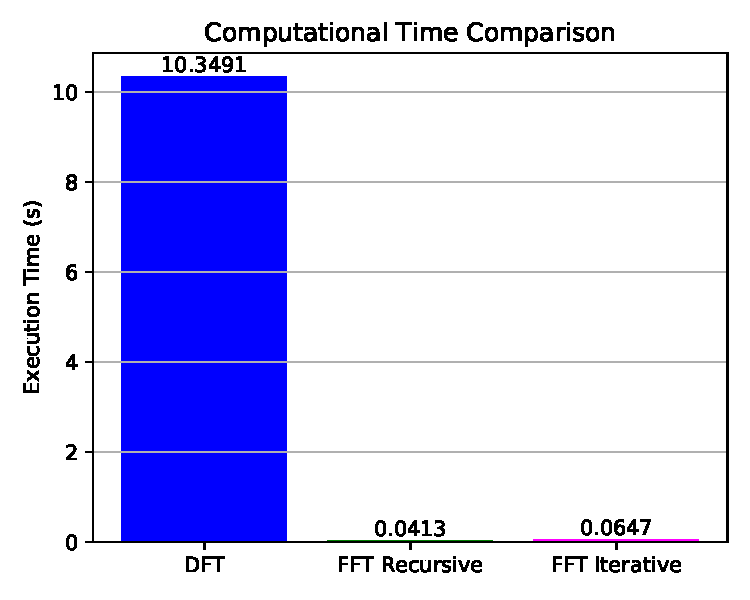
\includegraphics[width=0.45\textwidth]{figures/computional_time.pdf}
	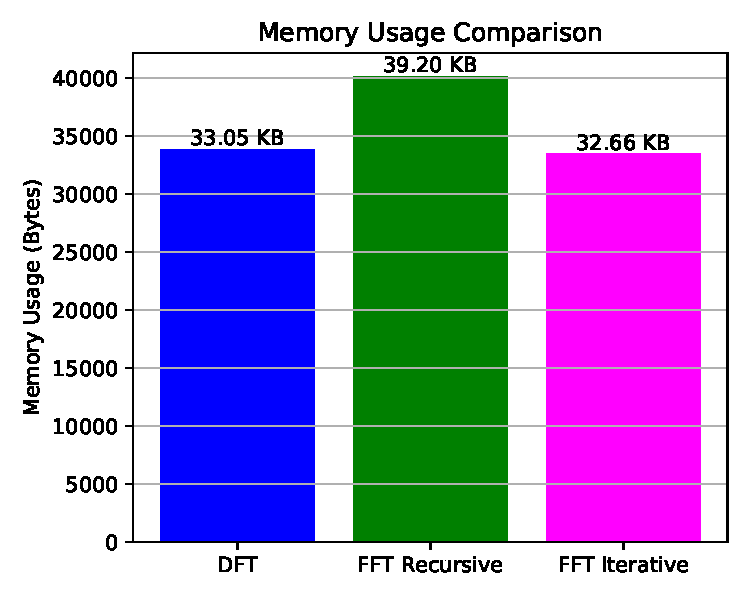
\includegraphics[width=0.45\textwidth]{figures/memory_usage.pdf}
	\caption{Computational time for fixed signal length (left). Memory usage comparison (right).}
	\label{fig:time_memory_comparison}
\end{figure}

\noindent Figure \ref{fig:scaling_comparison} examines how execution time and memory usage scale with increasing signal length. The execution time for the \ac{DFT} grows quadratically, whereas the \ac{FFT} scales logarithmically. Memory usage increases quadratically for the \ac{DFT} as well as for both \ac{FFT} methods. Nevertheless, the iterative \ac{FFT} outperforms the other methods in this scenario.

\begin{figure}[h!]
	\centering
	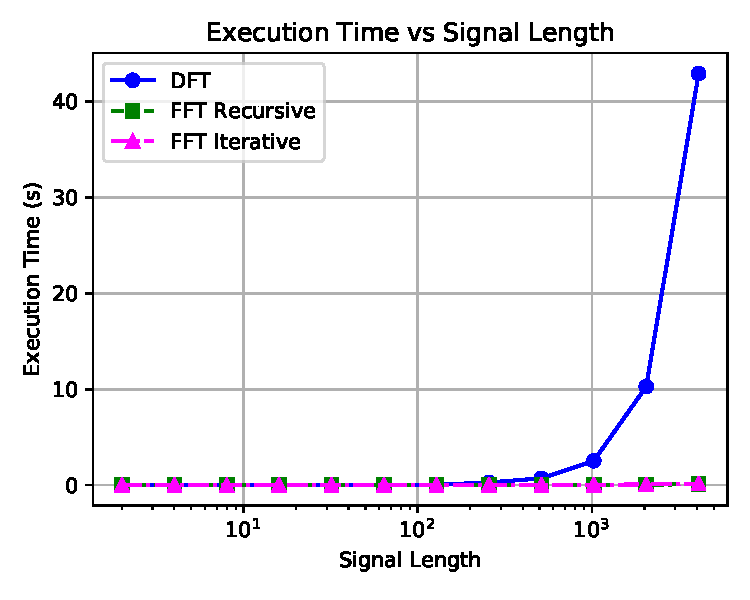
\includegraphics[width=0.45\textwidth]{figures/computional_time_cmp.pdf}
	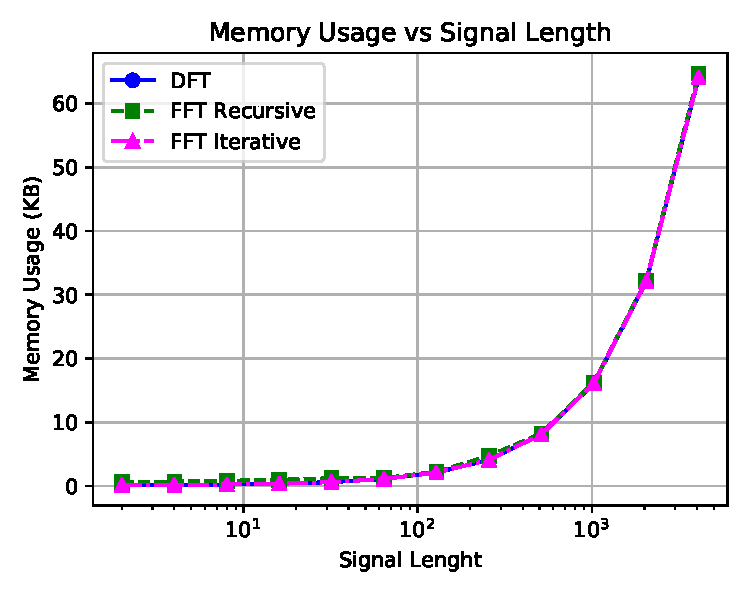
\includegraphics[width=0.45\textwidth]{figures/memory_usage_cmp.pdf}
	\caption{Execution time vs. signal length (left). Memory usage vs. signal length (right).}
	\label{fig:scaling_comparison}
\end{figure}

\subsection{Issues during Development}
When the performance tests of the \ac{FFT} were conducted, issues with the implementation of the iterative algorithm surfaced. It allocated more than twice as much data a the \ac{DFT} and recursive \ac{FFT} and was significantly slower than the recursive algorithm. The problem was the bit inversion of the signal, where a string-based approach and a copy of the original signal have been used.\\
After changing this the iterative \ac{FFT} requires the least data of all implementations and is almost as fast as the recursive \ac{FFT}.
Usually the iterative algorithm should be faster than the recursive one, which was not achieved.\\
Further tries of improving the algorithm did not lead to a faster computation time.
As that is only a slight performance issue and does not effect the overall functionality, the issue is neglected.

\section{Modulation and Demodulation (Non- and Quadrature)}

\subsection{Implementation Overview}
Modulation and demodulation are essential processes for signal transformation during transmission and recovery. The implementation includes non-quadrature and quadrature approaches, as defined in the Python script \texttt{modulation.py}. Non-quadrature modulation multiplies the input signal with a cosine function of a given modulation frequency, effectively shifting the signal in the frequency domain. Demodulation reverses this process by multiplying the modulated signal with twice the cosine function to recover the original signal. Quadrature modulation extends this concept by combining two input signals, one modulated with a cosine function and the other with a sine function, enabling dual-channel transmission. The quadrature demodulation separates these two components to recover the original signals.

\subsection{Purpose and Testing}
The \texttt{modulation.py} implementation is validated in the test script \texttt{test\_modulation.py}, which covers various modulation and demodulation scenarios. For the \texttt{modulate} function, tests verify that the modulated signal aligns with expected cosine-modulated values for a range of input frequencies and amplitudes. The \texttt{demodulate} function is tested to ensure it accurately reconstructs the original signal after modulation and demodulation.\\
Quadrature modulation and demodulation undergo specific tests to confirm the proper separation and scaling of the two orthogonally modulated signals during demodulation. The tests include scenarios with independent input signals as well as edge cases, such as all-zero inputs or constant signals, to ensure numerical stability and accuracy. Each test employs assertions and comparisons against expected outcomes to validate the functionality and robustness of the methods.

\subsection{Visualization of Modulation Processes}
The script \texttt{vis\_modulation.py} provides visual insights into the modulation and demodulation processes. Figure \ref{fig:modulation_visualizations} illustrates these processes. The left panel shows the original, modulated, and demodulated signals for the non-quadrature case. Modulated signals are visibly shifted and scaled, while demodulated signals closely match the originals. The right panel depicts quadrature modulation and demodulation, highlighting the successful separation and reconstruction of two orthogonal signal components. These visualizations confirm the implementation's correctness and reliability.

\begin{figure}[h!]
	\centering
	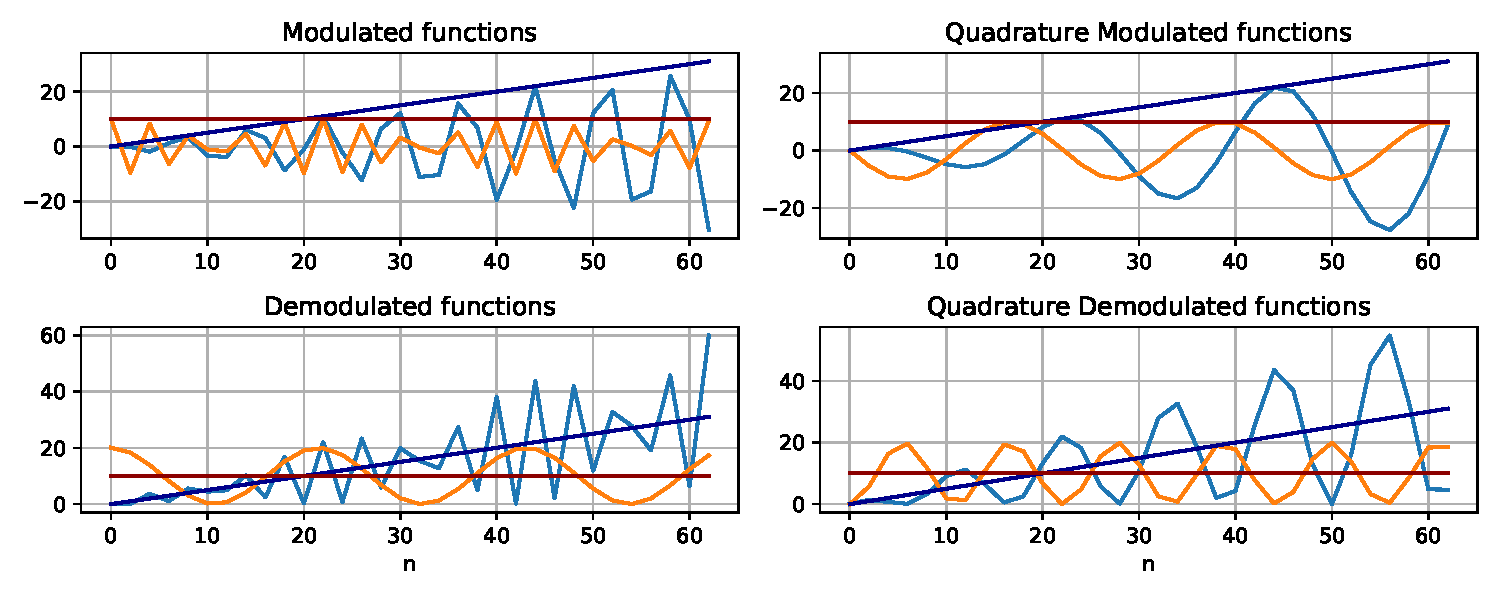
\includegraphics[width=0.75\textwidth]{figures/modulation.pdf}
	\caption{Non-quadrature modulation and demodulation (left). Quadrature modulation and demodulation (right).}
	\label{fig:modulation_visualizations}
\end{figure}

\section{Convolution}
Convolution is implemented in time-domain (\texttt{/module/convolution.py})
and as fast convolution using the \ac{FFT} (\texttt{/module/fast\_convolution.py}).
To verify the correctness of the implementations,
a sawtooth signal is convolved with a shifted impulse signal.
The results are the same for both implementations within a tolerance smaller than \(\pm10^{-15}\).
When convolving with a shifted impulse signal, the convolution is equal to the shifted signal.
This is shown in Figure \ref{fig:convolution}.
\begin{figure}[h!]
	\centering
	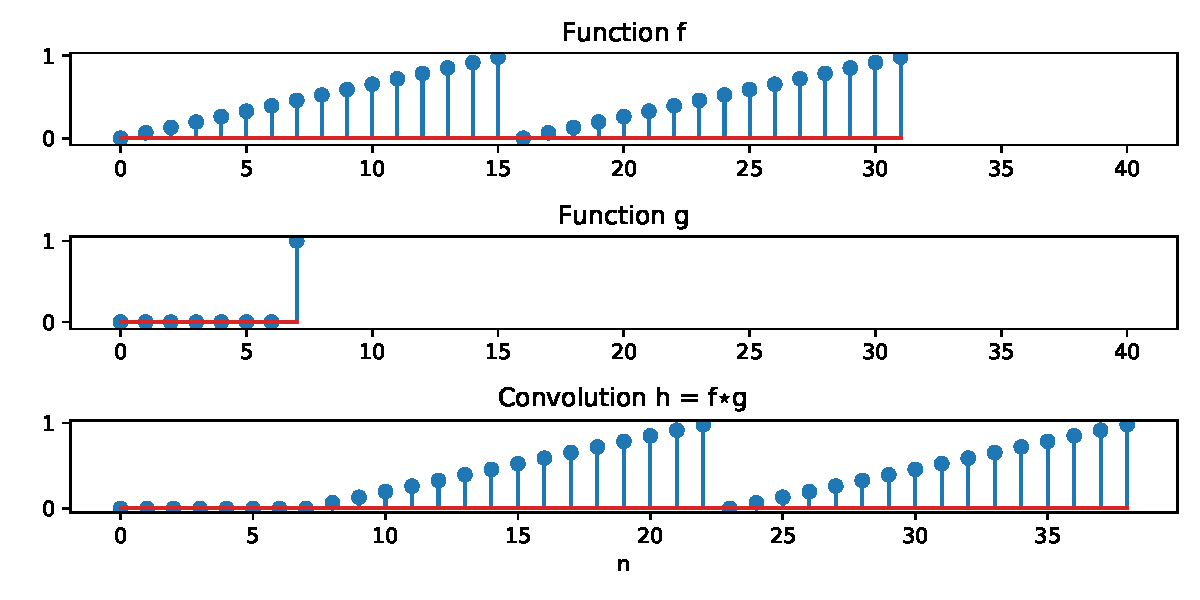
\includegraphics[width=0.6\textwidth]{figures/convolution.pdf}
	\caption{Convolution of a sawtooth signal with a shifted impulse signal.}
	\label{fig:convolution}
\end{figure}

\section{Low-Pass Filter}

The filter is implemented in \texttt{/module/low\_pass\_filter.py}.
By convolving the input signal with the filter function of length \(N\),
the signal is low-pass filtered.

\begin{figure}[h!]
	\centering
	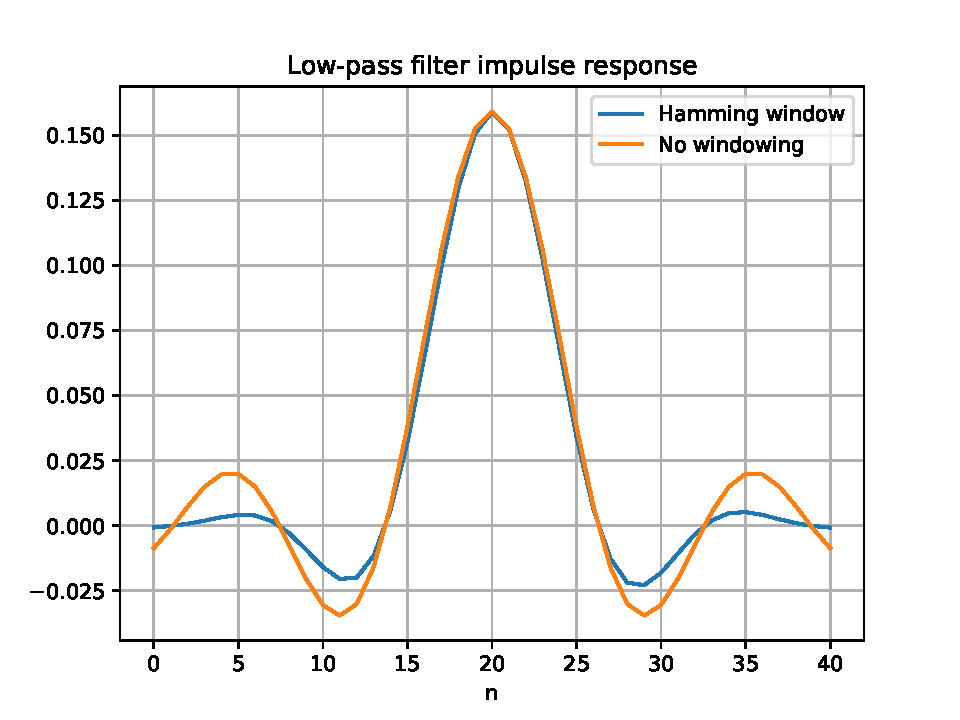
\includegraphics[width=0.45\textwidth]{figures/impulse_response.pdf}
	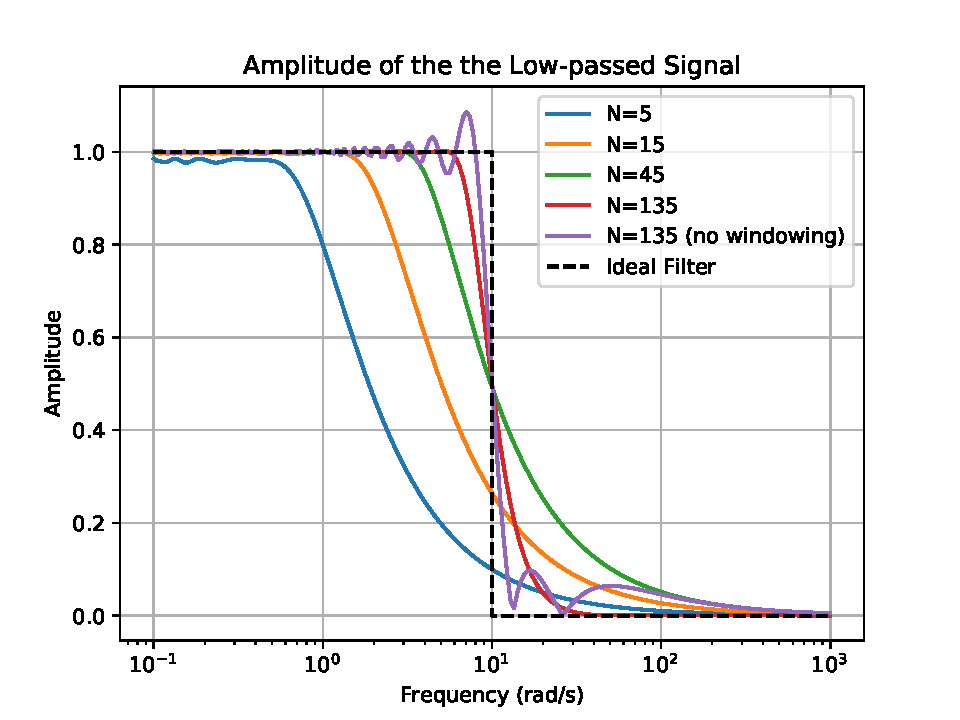
\includegraphics[width=0.45\textwidth]{figures/passband.pdf}
	\caption{Impulse response of the low-pass filter with N=20 (left). Amplitude of the low-passed signal with different filter lengths (right).}
	\label{fig:low_pass_filter}
\end{figure}
\noindent As filter function, a \(sinc\) function with applied Hamming windowing is used. Figure \ref{fig:low_pass_filter} (left) shows the impulse response with and without a Hamming window. It can be observed that the Hamming window reduces the ripples at the beginning and end of the impulse response.\\
The frequency response of the low-pass filter is determined by filtering cosine waves with increasing frequencies and calculating the highest amplitude of the output signal. This is shown for different filter lengths in Figure \ref{fig:low_pass_filter} (right). Here, the cut-off frequency is 10 \({rad}/s\).
It can be observed that the steepness of the transition band increases with the filter length. If no Hamming window is applied, there are ripples in the passband and the stopband.\\
The performance of the low-pass filter highly depends on the implementation of the convolution. Table \ref{tab:timing_comparison} shows the timing comparison when using fast convolution and convolution in time-domain. For the given parameters, the fast convolution is on average more than 2.4 times faster then in time-domain.
\begin{table}[h!]
	\centering
	\begin{tabular}{|l|c|c|}
		\hline
		                   & \textbf{Fast Convolution} & \textbf{Time-Domain Convolution} \\ \hline
		Average time       & 0.2997 \(s\)              & 0.7241 \(s\)                     \\ \hline
		Standard deviation & 0.0397 \(s\)              & 0.0603 \(s\)                     \\ \hline
		Min time           & 0.2598 \(s\)              & 0.6684 \(s\)                     \\ \hline
		Max time           & 0.5171 \(s\)              & 1.269 \(s\)                      \\ \hline
		Median time        & 0.2864 \(s\)              & 0.715 \(s\)                      \\ \hline
	\end{tabular}
	\caption{Timing comparison for Low-Pass Filter using fast convolution and time-domain convolution. Function length = 20000, Filter length = 50, Number of tests = 200.}
	\label{tab:timing_comparison}
\end{table}

\chapter{Overall system}
The overall system recreates the transmission of two signals over a common medium using modulation. On the sender side, the signals are low-pass filtered, modulated and added. The sum of both modulated signals is then transmitted to the receiver,
where the signal is demodulated and low-pass filtered again.

\section{Testing with simple signals}
The file \texttt{project.py} contains the implementation of the overall system.
For testing, two simple signals are used. The first signal is a sum of cosine waves with different frequencies and phases (Equation 2.1) and the second signal is a sawtooth wave (Equation 2.2).
\begin{equation}
	f_1(t) = 3 + cos(t+1) + 2cos(3t+2) - 5cos(4t-1) + cos(13t)
\end{equation}
\begin{equation}
	f_2(t) = 3 \cdot (t\mod\pi)
\end{equation}
Both signals are sampled 32 times in the interval from 0 to 2\(\pi\). Each step of the transmission is shown in Figure \ref{fig:overall} (top), where the left side depicts the operations in time-domain and the right side in frequency-domain, by showing the magnitude of the first half of the Fourier coefficients. The low-pass filtered signals are compared to the reconstructed signals in the bottom figure.\\
The cut-off frequency is choosen to be \(\omega_c=\) 7 \(rad/s\). As seen in the second row, the low-pass filter removes the high frequency components. Furthermore the sampling rate is increased by factor 2 after the low-pass filter, because modulation would not be possible without violating the sampling theorem. Then the signals are modulated with \(\omega_{mod_1}=\) 8 \(rad/s\) and \(\omega_{mod_2}=\) 23 \(rad/s\), so that their frequency bands do not overlap. After adding, demodulation and low-pass filtering, the reconstructed signals are nearly equal to the original, low-passed signals.\\
An alternative approach is to use quadrature modulation. This is shown in Figure \ref{fig:quadrature}, where the signals are modulated with the same modulation frequency \(\omega_{mod}=\) 8 \(rad/s\), but with a cosine and a sine wave, respectively.\\
When a overlap of the frequency bands is introduced, the signals cannot be reconstructed properly. For this example the signals are sampled 64 times.
The modulation frequencies are \(\omega_{mod_1}=\) 8 \(rad/s\) and \(\omega_{mod_2}=\) 19 \(rad/s\). This is shown in Figure \ref{fig:overlap},
where the signals contain noise of the other signal. Most significant is a noise in the sawtooth signal with a frequency of 7 \(rad/s\).

\section{Testing with sound files}

The overall system is also tested with sound files (\texttt{project\_soundfile.py}). The first sound file is a Jodler and the second a squeaking violin.
\begin{itemize}
	\item \texttt{soundfiles/Jodler.wav}
	\item \texttt{soundfiles/Violine.wav}
\end{itemize}
The sampling rate is \(f_s=\) 44100 \(Hz\), respectively \(w_s\approx\) 277088 \(rad/s\). The signals are low-pass filtered with a cut-off frequency \(\omega_c=\) 20000 \(rad/s\). The modulation frequencies are \(\omega_{mod_1}=\) 25000 \(rad/s\) and \(\omega_{mod_2}=\) 70000 \(rad/s\). As the signals are well separated in the frequency domain and the sampling frequency is sufficient,
the reconstruction is successful. The soundfiles after each operation are saved in the \texttt{soundfiles} directory, in order to listen to the (intermediate) results. Figure \ref{fig:soundfiles} depicts the overall system with sound files.

\appendix

\chapter{Figures}
\pagenumbering{roman}
\setcounter{page}{3}

\begin{figure}[h!]
	\centering
	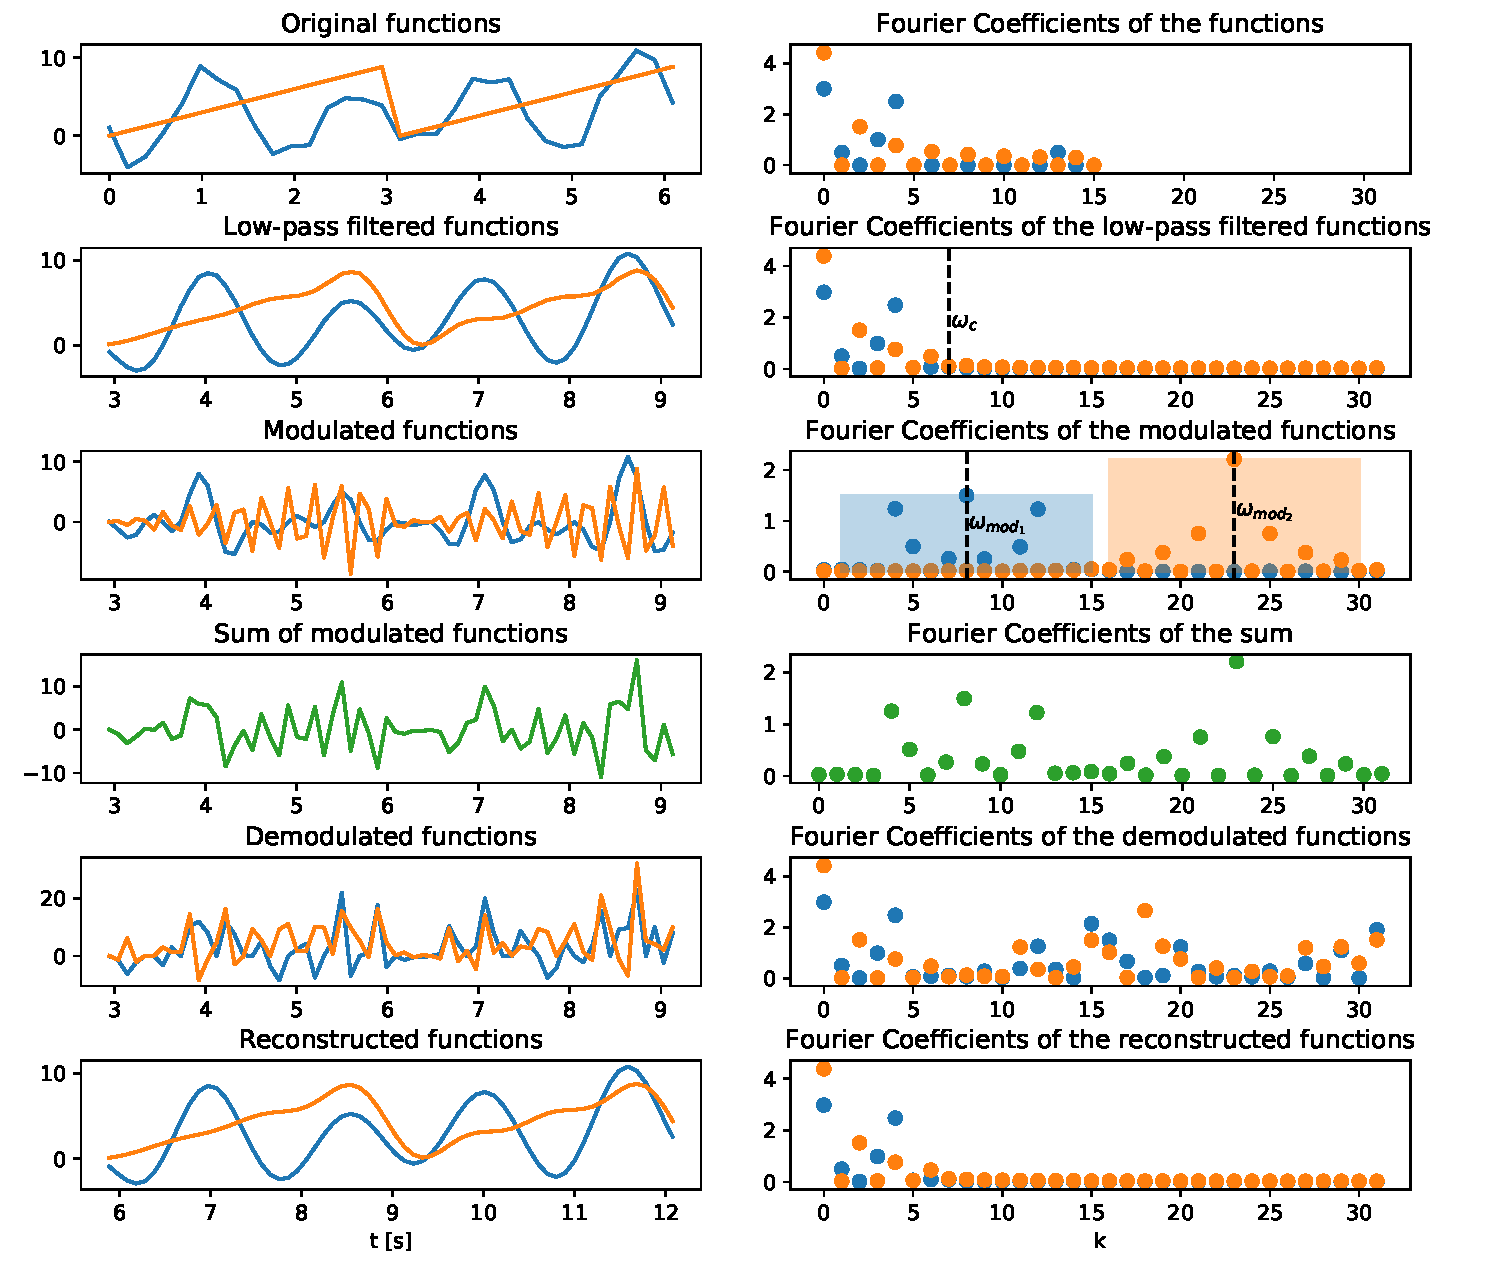
\includegraphics[width=\textwidth]{figures/overall_sampling.pdf}
	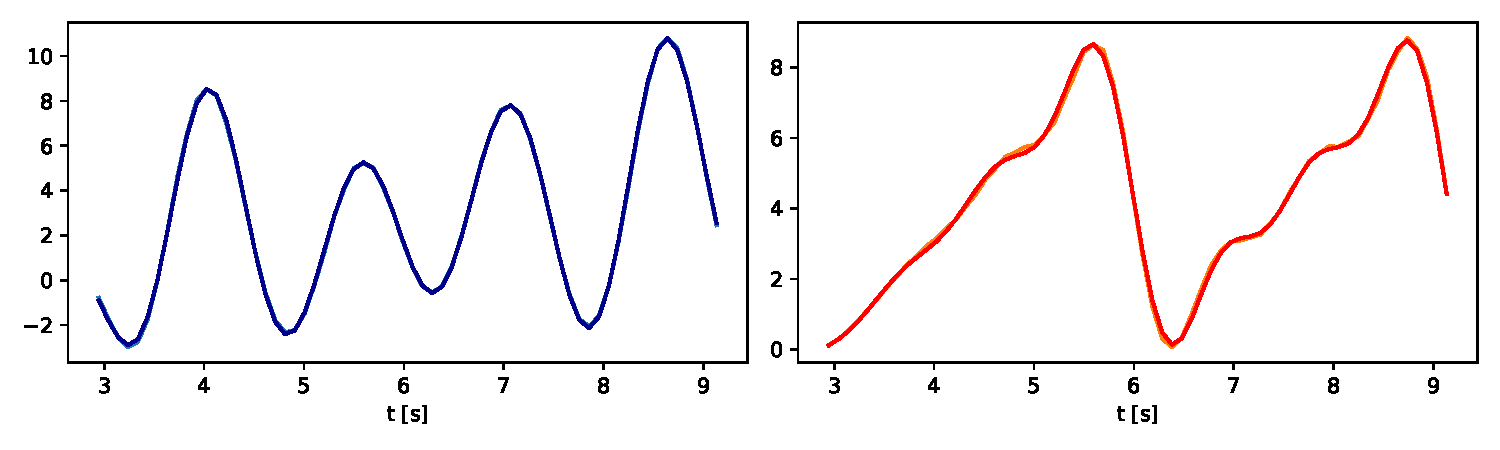
\includegraphics[width=0.9\textwidth]{figures/sampling_cmp.pdf}
	\caption{Overall sytsem (top). Reconstructed vs. low-pass filtered signals (bottom).}
	\label{fig:overall}
\end{figure}


\begin{figure}[h!]
	\centering
	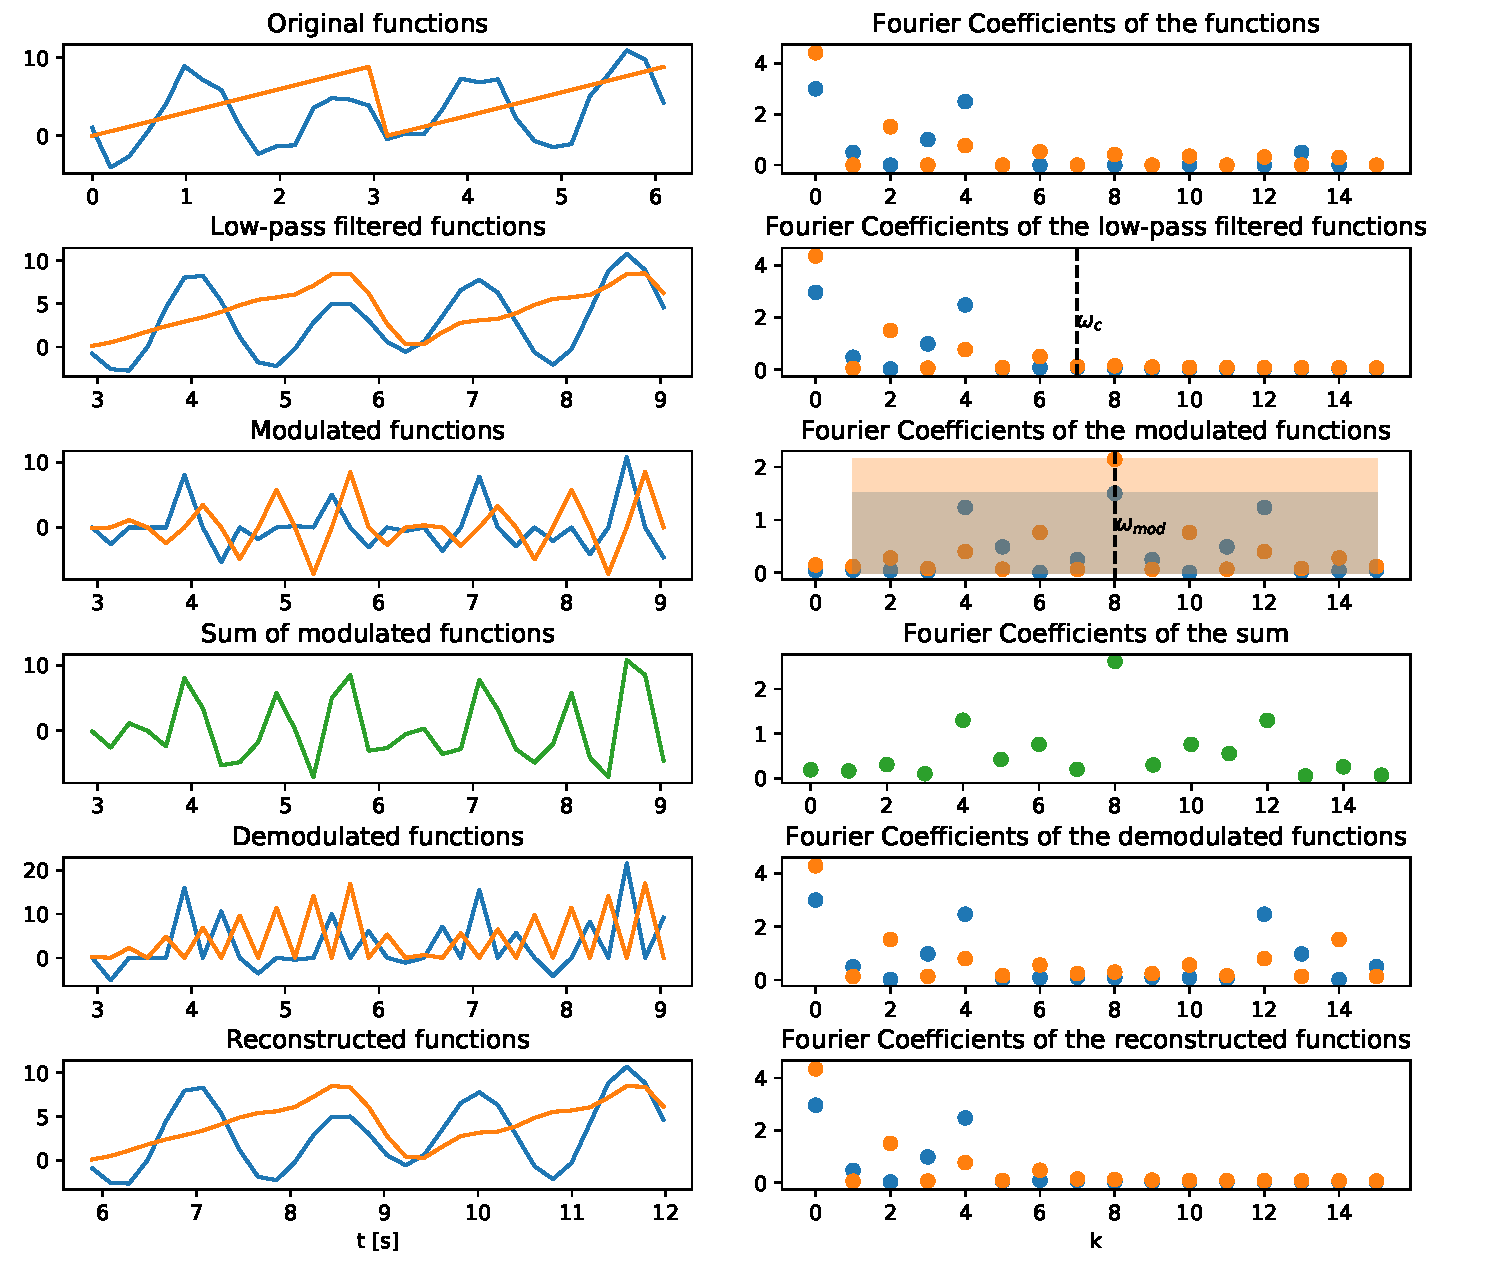
\includegraphics[width=\textwidth]{figures/overall_quad.pdf}
	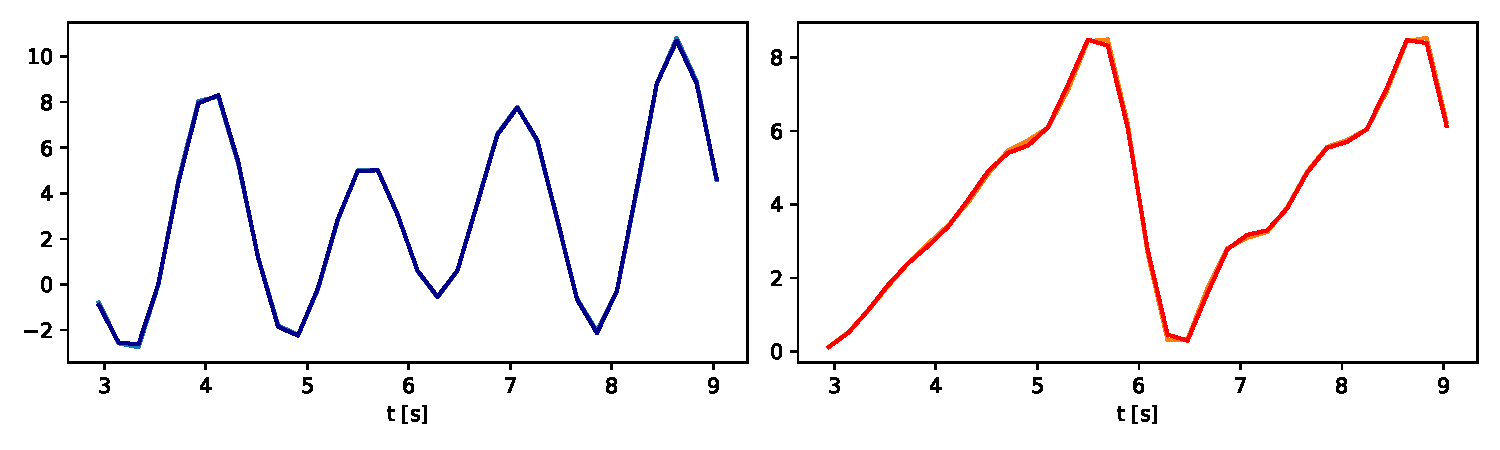
\includegraphics[width=0.9\textwidth]{figures/quad_cmp.pdf}
	\caption{Overall sytsem with quadrature modulation (top). Reconstructed vs. low-pass filtered signals (bottom).}
	\label{fig:quadrature}
\end{figure}

\begin{figure}[h!]
	\centering
	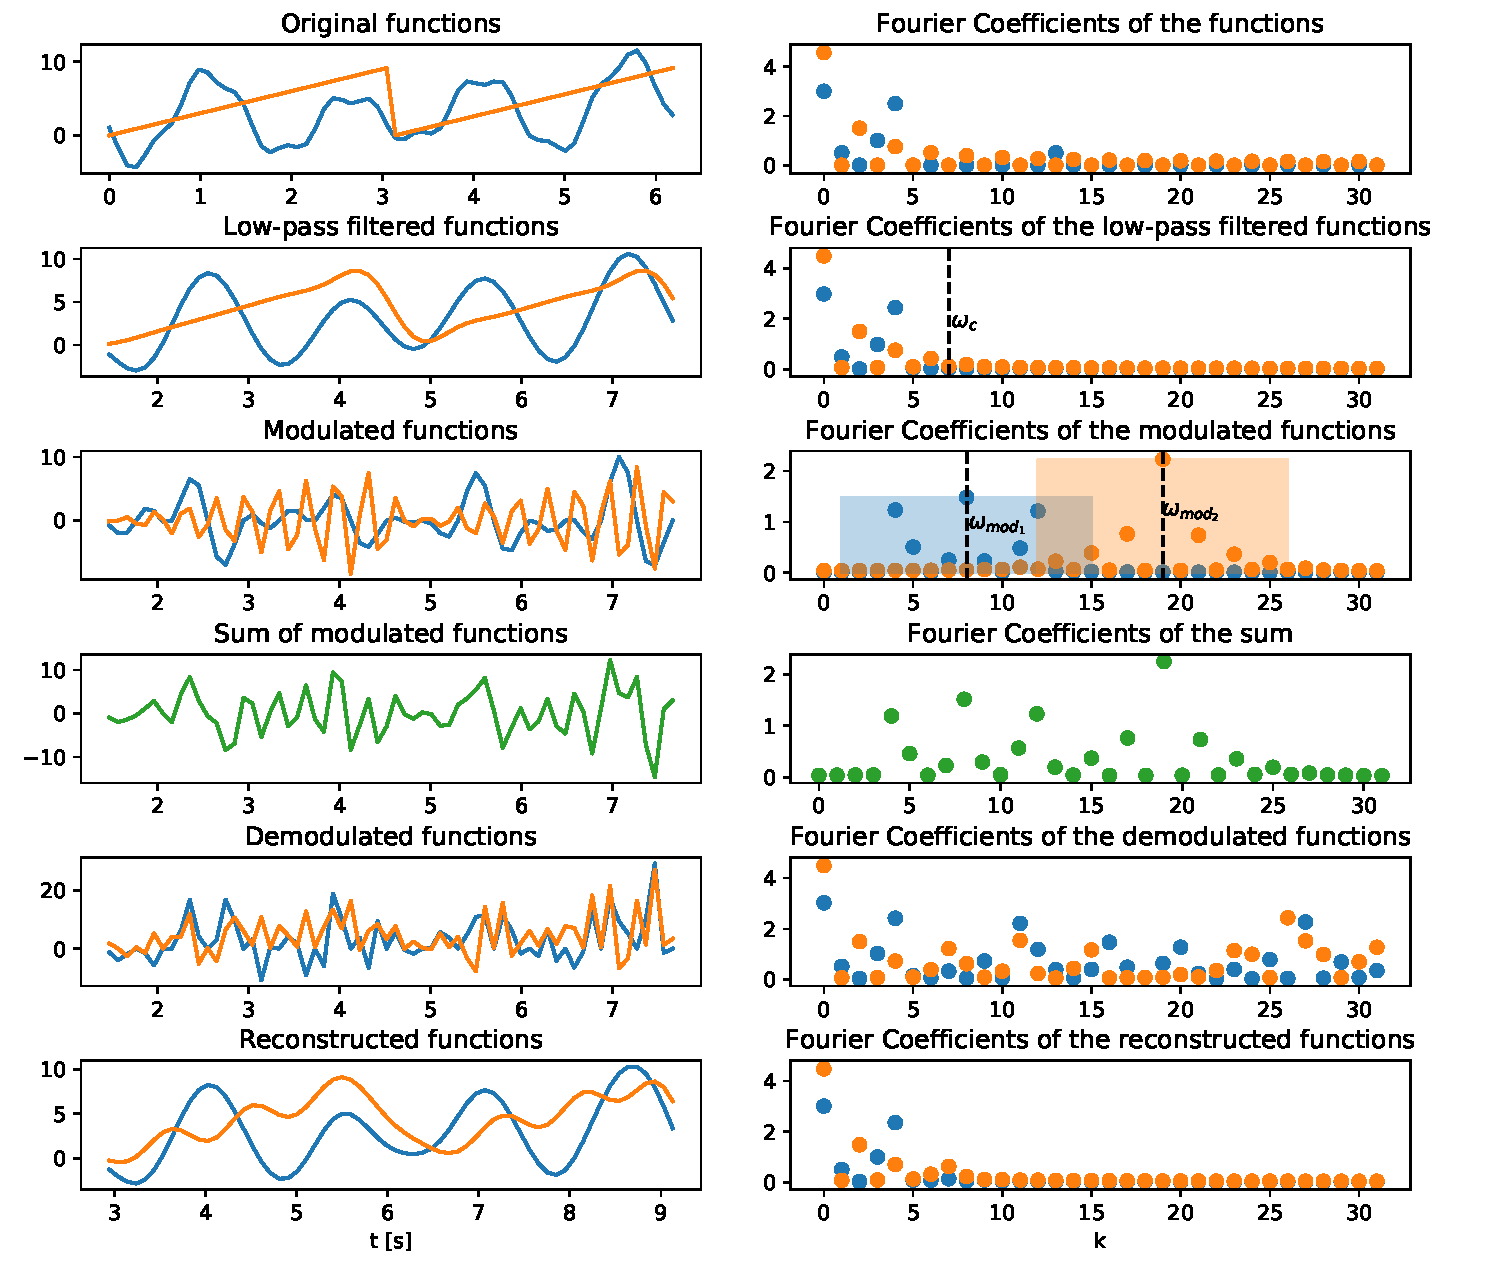
\includegraphics[width=\textwidth]{figures/overall_overlapping.pdf}
	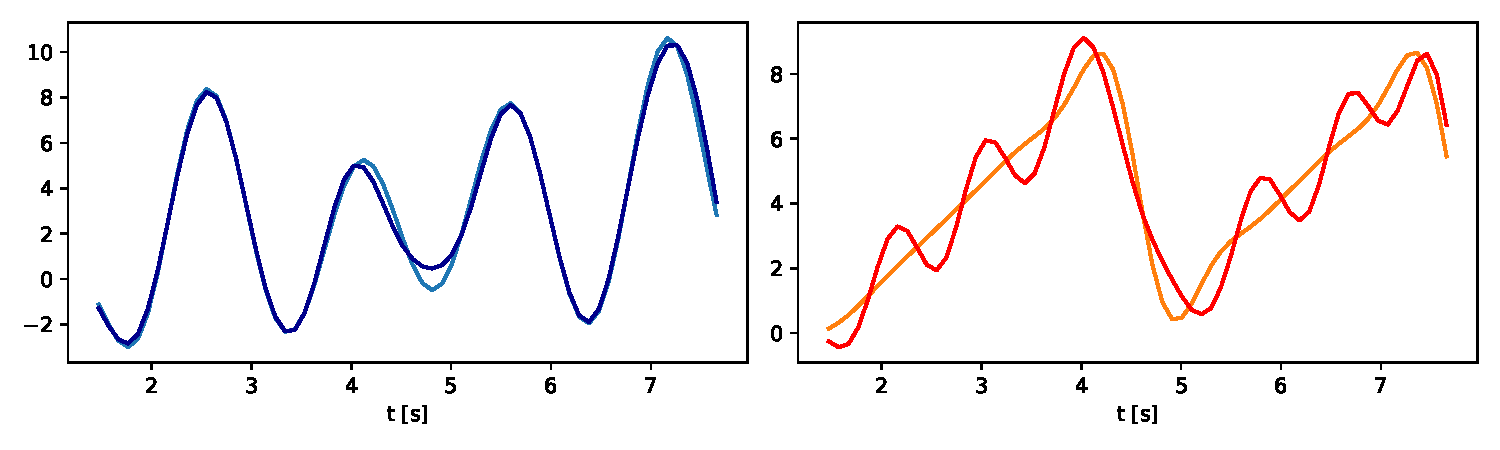
\includegraphics[width=0.9\textwidth]{figures/overlapping_cmp.pdf}
	\caption{Overall sytsem with overlapping frequency bands (top). Reconstructed vs. low-pass filtered signals (bottom).}
	\label{fig:overlap}
\end{figure}

\begin{figure}[h!]
	\centering
	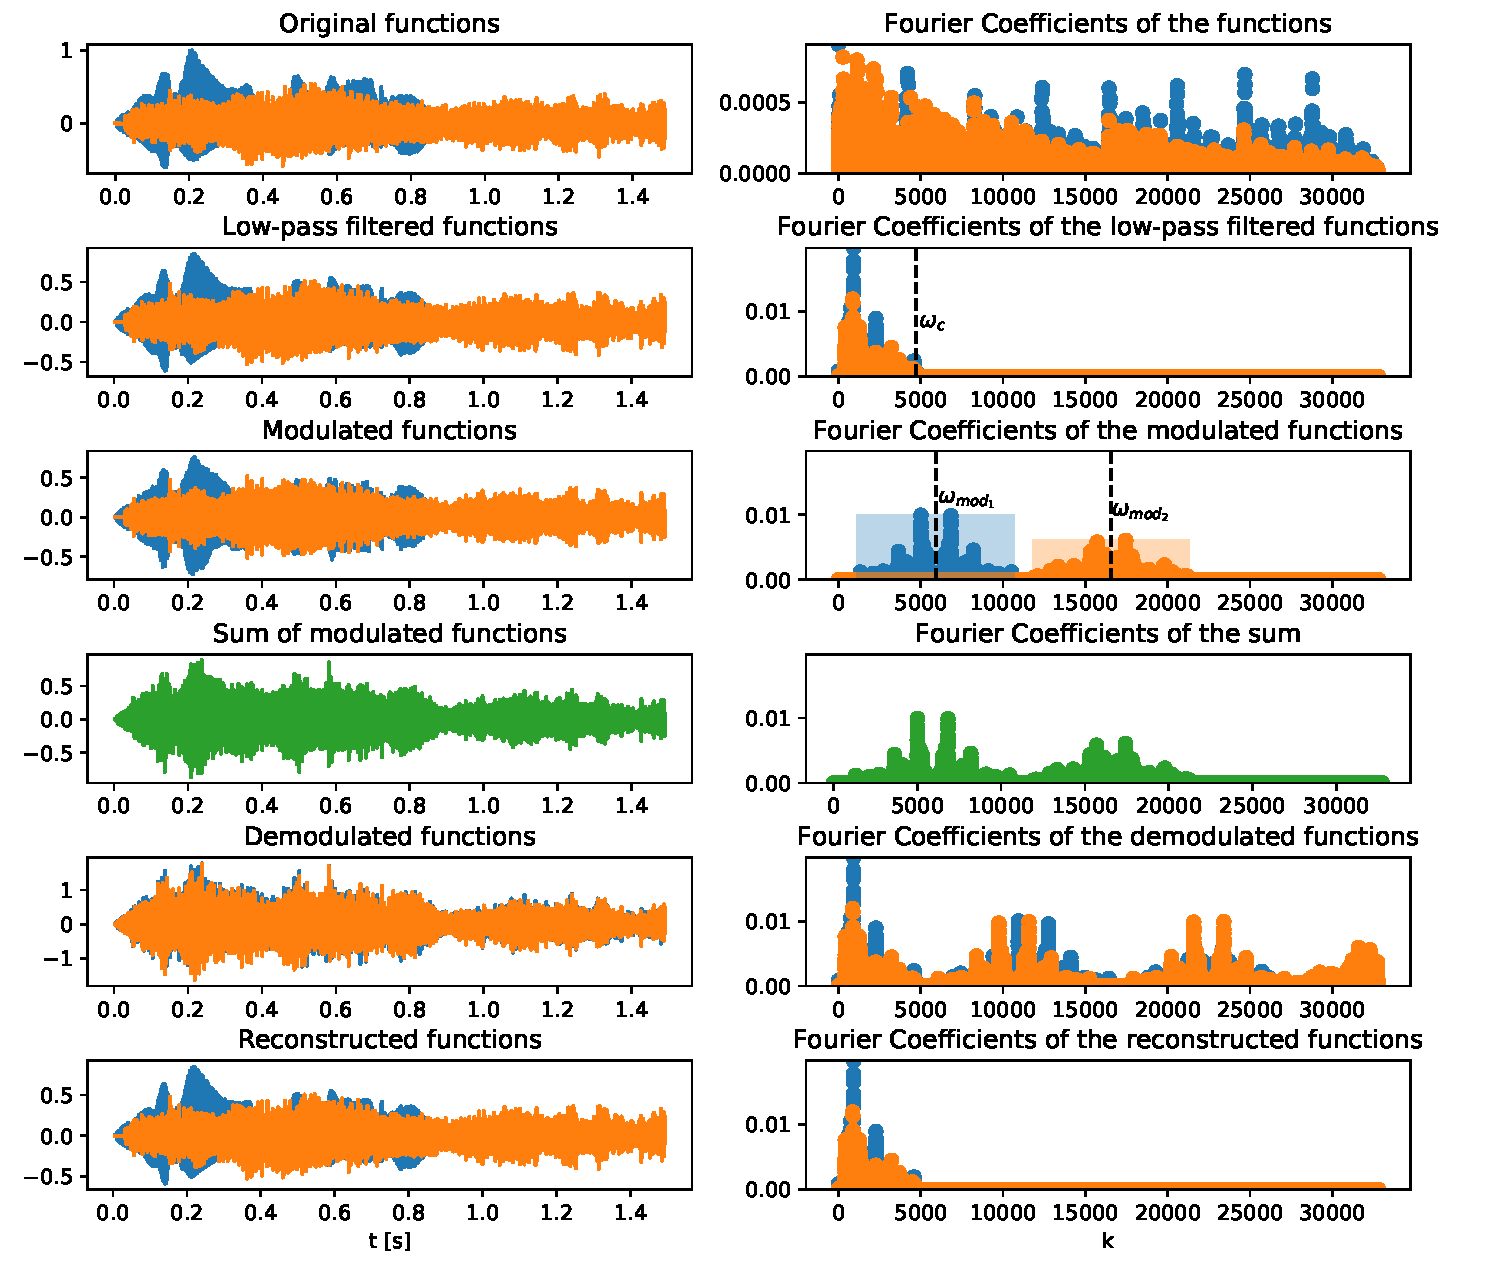
\includegraphics[width=0.9\textwidth]{figures/overall_soundfile.pdf}
	\caption{Overall system with sound files.}
	\label{fig:soundfiles}
\end{figure}

\end{document}
